% !Mode:: "TeX:UTF-8"
\documentclass[master]{bnuthesis}
% \documentclass[%
%   bachelor|master|doctor, % mandatory option
%   xetex|pdftex|dvips|dvipdfm, % optional
%   openany|operight,  % 连续页面,或者右侧打开
%   secret,  % 是否涉密
%   arialtoc,arialtitle]{bnuthesis}

% 所有其它可能用到的包都统一放在这里,可以根据实际需要添加或者删除。
\usepackage{bnutils}
\usepackage[table]{xcolor}
% 你可以在这里修改配置文件中的定义,导言区可以使用中文。
% \def\myname{薛瑞尼}

\begin{document}
% 定义所有的eps文件在figures子目录下
\graphicspath{{figures/}}

%%% 封面部分
\frontmatter
% !Mode:: "TeX:UTF-8"
%%% Local Variables:
%%% mode: latex
%%% TeX-master: t
%%% End:
%\secretlevel{绝密} \secretyear{10}


\ctitle{基于关系路径的知识库补全算法研究}
%\makeatletter
%\cdegree{博士}

\makeatother

%\makeatletter
%\cdegree{博士}

\makeatother

\cauthor{黄勇}
\csupervisor{王志春\;副教授 \\ \hspace*{6em}}
\cdepartment[]{计算机软件与理论} 
\cmajor{知识工程}
\cnum{201521210022}
\cdate{\the\year  年 \the\month 月}

\etitle{Knowledge Base Completion by relational path methods}

% 定义中英文摘要和关键字
\begin{cabstract}
  知识库通常从非结构化、半结构化的数据中抽取事实,构建结构化的知识,常用三元组进行存储表示。知识库在信息检索、问答系统和人工智能等不同领域具有重要作用,尽管当前有很多大规模知识库如Freebase、YAGO包含大量三元组,但这些知识库中的三元组是不完备的,很多实体对之间的关系存在缺失。 
  知识库补全基于现有知识库的三元组,预测知识库中实体和实体之间的关系。
  当前的知识库补全算法主要包括基于符号逻辑的知识库补全算法和基于表示学习的知识库补全算法,
  其中一种典型的基于符号逻辑的知识库补全算法是\textbf{路径排序算法}。路径排序算法抽取
  实体之间的\textbf{关系路径特征},构建逻辑回归分类模型,对知识库中实体和实体之间关系进行预测。

  当前路径排序算法基于关系路径进行知识库补全,并没有考虑实体和实体之间的属性特征关系,一些知识库补全系统构建的正负实例对比例悬殊,进行模型训练很难抽取有效的路径特征,也难以进行模型训练,如何构建更丰富有效的特征类型,学习更有效的模型,任然是知识库补全的重要任务。
  本论文在传统的关系路径特征基础上,提出了一种新的结合关系路径特征和\textbf{实体属性特征}知识库补全模型,并将不同类型的关系路径特征、实体属性特征进行组合,显著提升了知识库补全效果。
  考虑到知识库补全中正负例不平衡问题,为了获得更好的模型预测结果,在传统逻辑回归模型的基础上,本研究基于\textbf{学习排序模型}的知识库补全,通过学习排序损失函数,优化正负实体对的排序,从而提高知识库补全模型效果。本论文的研究创新点主要有:
  \begin{itemize}[$\bullet$]
    \item 抽取关系路径和实体属性特征作为知识库补全的特征,将多种不同类型特征进行组合,极大拓展了知识库补全系统的维度,增强了知识库补全效果。
    \item 基于学习排序算法预测知识库补全中实体和实体的关系,通过直接学习知识库补全中的实体对排序顺序,改进损失函数进行模型预测。
    \item 构建基于逻辑回归、学习排序树模型方法的知识库补全模型,通过候选实体对生成,模型排序,利用不同知识库数据特征选择合适的排序模型。
  \end{itemize}
\end{cabstract}

\ckeywords{知识库补全,路径排序算法, 学习排序模型,关系路径特征,实体属性特征}

\begin{eabstract}
Knowledge base (KB) completion aims to predict new facts
from the existing ones in KBs. There are many KB completion approaches,
one of the state-of-art approaches is Path Ranking Algorithm
(PRA), which predicts new facts based on relational path types connecting entities.
PRA takes the relation prediction as a classification problem, and
logistic regression or SVM is used as the classification model. In this paper, our model
use both literal facts and relational path types as feature matrix, which is much more comprehensive and complicated. We
consider the relation prediction as a ranking problem, learning to rank
model is trained on relations to predict new facts. Besides. We propose to extract literal features from literal facts, and incorporate them with path-based
features extracted from relational facts; predictive
model is then trained to infer new
facts with assembly features and bring higher precision scores in classification metrics and ranking metrics. Experiments on YAGO show that our proposed approach outperforms approaches using relational path features and classification models.
This paper has three main contribution, including:
\begin{itemize}[$\bullet$]
    \item KB completion feature type is comprehensive including both relational path and literal features to generate feature matrix, and in different KBs our features help to generate higher scores both in ranking tasks and classification tasks.
    \item KB completion was considered as a ranking method, we use learning to ranking model to rank entity pairs rather than simple taking it as a classification model.
    \item KB completion methods are easily explainable, with combined literal and relational facts we can easily predict relation in KBs, tree models are used with assembly features, this helps us to rank entity pairs in different.
  \end{itemize}

\end{eabstract}

\ekeywords{Knowledge Base Completion, Learning to Rank, Path Ranking, Relational Path}

\makecover

% 目录
\tableofcontents

% 符号对照表
% % !Mode:: "TeX:UTF-8"
\begin{denotation}

\item[HPC] 高性能计算 (High Performance Computing)
\item[cluster] 集群
\item[Itanium] 安腾
\item[SMP] 对称多处理
\item[API] 应用程序编程接口
\item[PI]	聚酰亚胺
\item[MPI]	聚酰亚胺模型化合物,N-苯基邻苯酰亚胺
\item[PBI]	聚苯并咪唑
\item[MPBI]	聚苯并咪唑模型化合物,N-苯基苯并咪唑
\item[PY]	聚吡咙
\item[PMDA-BDA]	均苯四酸二酐与联苯四胺合成的聚吡咙薄膜
\item[$\Delta G$]  	活化自由能~(Activation Free Energy)
\item [$\chi$] 传输系数~(Transmission Coefficient)
\item[$E$] 能量
\item[$m$] 质量
\item[$c$] 光速
\item[$P$] 概率
\item[$T$] 时间
\item[$v$] 速度
\end{denotation}

% 插图索引
%\listoffigures
% 表格索引
%\listoftables

%%% 正文部分
\mainmatter
% !Mode:: "TeX:UTF-8"
%%% Local Variables:
%%% mode: latex
%%% TeX-master: t
%%% End:

% 绪论和个人工作

\chapter{绪论}
\label{cha:intro}
近些年来,随着互联网的快速发展,人工智能和大数据技术的兴起和应用,网络数据、信息和知识大量增长。
传统的基于网页链接检索的信息存储、信息检索方式越来越难于进行查找学习知识,随着移动设备
的增加,人们对于信息检索、知识获取的要求也越来越高,面对各种数据信息,
人们查找检索知识的需求越来越迫切,越来越期望能更好更快的检索了解学习知识。
随之知识库构建、推理和应用变得流行起来,越来越多的大学、科研机构和商业公司开始构建大规模知识库,如Google Knowledge Graph\cite{Dong},NELL\cite{NELL-aaai15},YAGO\cite{Suchanek:2007:YCS:1242572.1242667},
Freebase\cite{Bollacker2008FreebaseAC},DBpedia\cite{Bizer:2009:DCP:1640541.1640848}等。
这些知识库基于自动和半自动的信息抽取、众包、专家领域内知识等进行构建,
把互联网、书籍、数据库等各处非结构化的文本中数据结构化、抽取构建知识库,
获得了大量的实体、关系和属性信息,能为人们提供的方便快捷的信息查询、检索、知识学习途径。
这类知识库的数据完整性、数据精确性和数据质量等衡量指标非常高,
已经有很多基于知识库的系统被成功用于商业领域,如谷歌搜索引擎\footnote{https://googleblog.blogspot.com/2012/05/introducing-knowledge-graph-things-not.html},
微软的必应搜索\footnote{https://blogs.bing.com/search/2013/03/21/understand-your-world-with-bing/}等。
除了这些通用领域的知识库之外,也有很多领域知识库被构建和应用,知识库也被用于生物学\cite{Dumontier:2014:BRL:2878453.2878554}、金融学、教育学等各个领域,一些较为成熟的问答系统、个人手机助手如Siri、Google Assistant、微软小冰等也将知识库集成其中。

图\ref{kb}是一个简单的知识库例子,常见的知识库可以用有向图进行逻辑上的可视化表示。
图中展示了实体、实体和实体之间关系,其中实体是描述现实中实际存在的事物、地点、人物、事件如:北京师范大学、北京等,关系是描述实体和实体之间存在的某种联系和特征,如北京师范大学和北京存在着位于的关系。除此之外,
一个知识库中的三元组还可以分为关系型三元组和实体属性三元组。关系三元组典型的例子如:北京师范大学,位于,北京。其中“北京师范大学”和“北京”是实体,
属性事实三元组如:北京,人口,2150万。
其中“北京”是实体,“2150万”是描述实体属性的属性值,“人口”是北京这类实体具有的一种属性类型。
通常关系型三元组用来描述实体和实体之间的联系,实体属性三元组描述实体的属性事实特征,这些不同类型的三元组共同构成一个完整的知识库。

\begin{figure}[H]
\begin{center}
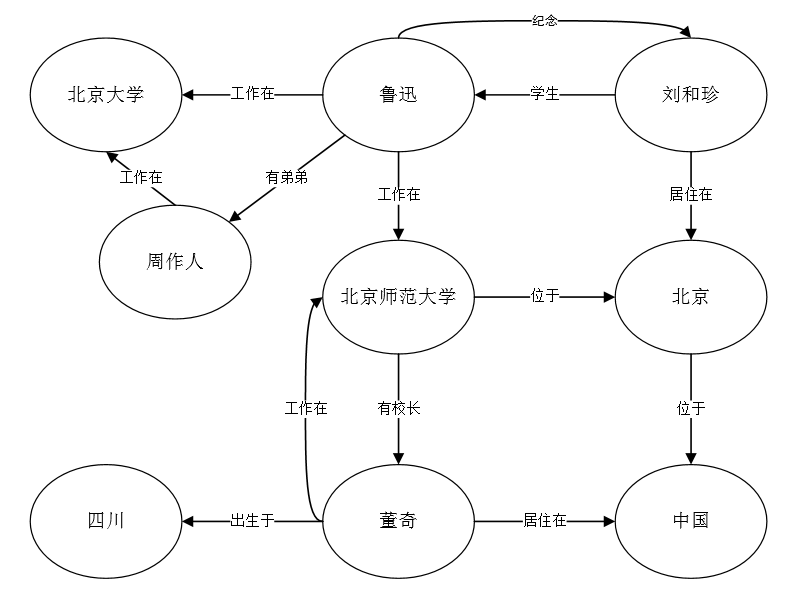
\includegraphics [width=0.5\textwidth]{kb.png}
\caption{一个知识库例子}
\label{kb}
\end{center}
\end{figure}

当前知识库相关的研究主要分为三个方面:(1)知识库的构建,各种基于互联网的、通用的、领域内的知识库构建。
(2)关系机器学习,基于已经构建好的知识库进行关系预测,知识库补全推理等。(3)知识库应用系统。如基于知识库的问答系统,
基于知识库的信息检索系统,生物、金融、教育等领域的本体知识库等。其中研究的热点之一就是知识库补全推理,即如何发掘知识库图结构中隐藏的关系。

当前存在的知识库系统如NELL、Knowledge Vault等,尽管已经包含了大量的实体、关系和属性,但这类知识库中很多实体和实体之间的关系任然是缺失的。例如,尽管知识库中存在很多三元组如:北师大,位于,北京;北京,位于,中国。但是当预测北师大是否位于中国时,通常计算机很难直接进行这类常识性的推理。如何构建一个辅助计算机进行常识推理系统,发现知识库中隐藏的实体和实体之间的关系,是知识库补全系统的重要任务之一。很多基于表示学习和基于符号逻辑的知识库补全算法被提出,这类算法都是基于知识库中现有的关系类型去预测知识库中未知的关系。但是在知识库中存在大量的属性事实型三元组未被使用,而这些属性事实三元组在进行关系预测时有很重要的作用,如:A,isMarriedTo,B,A,HasChild,C。当预测B是否是C的父母时,这些相关实体的年龄、性别等实体属性也很重要。

在构建知识库补全系统的过程中,基于符号逻辑的算法通常通过训练一个二分类的分类器来判断实体和实体之间是否具有某种关系。通常这个分类器的正例是通过抽取现有知识库中存在的三元组作为正例,或称之为正例三元组,而负例则是采用随机采样等方法生成负例三元组。通常在知识库补全系统中,每个正例三元组可以获得上万种不同的负例三元组,如何解决正负例三元组不均衡的问题,正确预测实体和实体之间的关系,也是知识库补全算法的一个重要优化方向。

\section{知识库构建}
在知识库构建过程中,数据完整性、数据精确性和数据质量是构建知识库的重要指标,
通常知识库可以由三元组组成。知识库的构建可以有多种方法:
(1)通过机器学习和自然语言处理技术自动抽取三元组\cite{Weikum2010FromIT}进行构建。
(2)半自动抽取的方法,通过从维基百科等网站的infobox基于规则模式抽取三元组。
(3)基于协同创作\cite{Vrandecic2014WikidataAF}的方法,通过众包的形式系统创建知识库。
(4)基于专家知识构建的领域内知识图谱,这些领域知识图谱有较高的专业性。

\subsection{YAGO知识库}
YAGO是一个从维基百科上抽取的、包含地理名词、WordNet\cite{Kasneci2008TheYA}等数据的知识库。
YAGO将WordNet的词汇定义与维基百科的分类体系进行了融合集成\cite{Suchanek2008YAGOAL},使得YAGO具有更加丰富的实体分类体系。YAGO还考虑了时间和空间知识\cite{Hoffart2011YAGO2EA},为很多知识条目增加了时间和空间维度的属性描述。目前,YAGO包含1.2亿条结合关系三元组和实体属性三元组的知识。YAGO也是IBM Watson\cite{Ferrucci2010BuildingWA}的后端知识库之一。
YAGO2\cite{Hoffart2013YAGO2AS}是YAGO的一个实例,当前YAGO2包括超过260万的实体和超过1.2亿的关系三元组知识,我们使用了其中实体的关系型三元组和属性型三元组共有4,484,914条、
37种关系型三元组的事实描述,同时有3,353,659条、35种属性性三元组的事实描述。

\subsection{Freebase知识库}
Freebase\cite{Bollacker2008FreebaseAC}是一个协同创作的知识库系统,内容通过用户添加,所有的条目采用结构化的形式,将结构分为三次:领域-类型-主题,其中,每一个条目叫做一个主题,每个主题包含不同的属性类型,一些同类型的主题组成一个类型,所有相关的类型构成一个领域。
这种通过协同创作方式创建了结构化的人类知识,截止2007年Freebase包含1.25亿条三元组,超过4000种类型和超过7000种属性知识。一些基于Freebase研究结构化知识的问答系统\cite{Yao2014InformationEO}\cite{Yao2015LeanQA},关注Freebase中的信息抽取和语义解析\cite{Yao2014FreebaseQI},也有一些研究关注Freebase中的实体消除歧义问题\cite{Zheng2012EntityDW}。

除了YAGO和Freebase知识库,也有很多重要的知识库如:Google Knowledge Graph,Wikidata,DBpedia等,这些通用的数据库都有着各自的特点和特色,表\ref{tab:addlabel-kb-list}展示了不同类型的知识库的实体、关系类型和三元组等数量,其中的M表示百万数量。本研究中的实验考虑到同时使用属性三元组和实体关系三元组,从而选择在YAGO和Freebase数据集中筛选属性特征较多的实体,
构建两个子数据集进行模型训练。

% Table generated by Excel2LaTeX from sheet '知识库'
\begin{table}[htbp]
  \centering
  \caption{不同知识库数据统计}
    \begin{tabular}{|l|l|r|l|}
    \hline
    知识库   & 实体数量  & \multicolumn{1}{l|}{关系类型数量} & 三元组数量 \\
    \hline
    Knowledge Graph & 570M  & 35000 & 18000M \\
    \hline
    YAGO2 & 9.8M  & 114   & 447M \\
    \hline
    DBpedia & 4.6M  & 1367  & 538M \\
    \hline
    wikidata & 18M   & 1632  & 66M \\
    \hline
    Freebase & 40M   & 35000 & 637M \\
    \hline
    \end{tabular}%
  \label{tab:addlabel-kb-list}%
\end{table}%


\section{知识库应用}
知识库在通过自动、半自动的信息抽取、专家知识构建知识库后,有着各种各样广泛的应用,
并能辅助人们检索、学习通用知识;一些专家对领域内的知识进行有序化,规范化,
辅助人们去了解学习一个领域的专业知识。

知识库最广泛的应用是谷歌和微软等商业公司的信息检索系统,2014年谷歌提出的知识图谱\cite{Dong2014KnowledgeVA}就是结合FreeBase、Wikidata以及各种互联网数据进行信息抽取,
知识整合后的著名系统,谷歌也在其博客上讲述了如何将知识库应用在实际的检索中,
微软的Satori也是一个类似的知识库系统,被必应搜索广泛应用。其他搜索公司如百度、搜狗等公司都在知识库构建和信息检索领域有各自的应用,
对于每一个用户搜索的关键词,我们可以通过知识库系统来返回更丰富,更全面的信息。比如搜索一个企业法人的姓名,我们的智能搜索引擎可以返回与这个人相关的所有历史借款记录、联系人信息、行为特征等。另外我们通过可视化把复杂的信息以非常直观的方式呈现出来, 使得用户对于对隐藏信息的来龙去脉一目了然。 

基于知识库的问答系统也有广泛的发展,2000年就有人提出基于知识的问答系统\cite{HERMJAKOB2000KnowledgeBasedQA},通过构架知识库完成问答。
也有很多方法基于知识库进行表示学习\cite{Yang2014JointRE},通过学习实体的低维度表示,学习知识库的实体和实体之间的关系,然后构建相关的知识库问答系统。
还有一些基于标签语义解析的方法,构建知识库问答系统\cite{Yih2016TheVO}。
一些论文\cite{Yu2017ImprovedNR}研究结合深度学习、关系抽取和问答系统,从而获得更好的知识库问答效果。
一些论文\cite{KeySun2016OpenKB}研究基于开放的知识库构建开放领域的问答系统,期望能基于百科知识进行问答系统构建。
也有基于知识库的系统通过结合智能计算\cite{Pandey2009KnowledgeAI},在医疗诊断领域获得一些突破。
也有一些研究结合了知识库和医疗图像信息\cite{Halpern2014EvaluationOC},对一些医疗疾病进行诊断治疗,期望能获得更好的治疗效果。

知识库在金融领域也可以有各种有效的应用。在进行金融风险检测时,
不一致性验证可以用来判断一个借款人的欺诈风险,这个跟交叉验证类似。比如借款人张三和借款人李四填写的是同一个公司电话,但张三填写的公司和李四填写的公司完全不一样,这就成了一个风险点,需要审核人员格外的注意。
除了贷前的风险控制,知识库也可以在贷后发挥其强大的作用。比如在贷后失联客户管理的问题上,知识图谱可以帮助我们挖掘出更多潜在的新的联系人,从而提高催收的成功率。

知识库也可以帮助我们分析用户和理解用户。通过结合多种数据源去分析实体之间的关系,从而对用户的行为有更好的理解。比如一个公司的市场经理用知识库来分析用户之间的关系,去发现一个组织的共同喜好,从而可以有针对性的对某一类人群制定营销策略。只有我们能更好的、更深入的理解用户的需求,我们才能更好地去做营销。

\section{知识库补全和推理}
虽然许多知识库的规模很大,但他们仍然是不完备的,如很多人的出生地点并未包含在知识库中,
一些演员是否出演过某些电影也是未知的。为了解决这个问题,很多知识库补全的方法被提出来,
这类方法基于知识库中已有的三元组预测新的三元组,如果将现有的知识库数据看做是多种关系构成的图,图的顶点是实体,图的边是实体对之间的关系,表\ref{tab:addlabel-relation}展示了YAGO和Freebase知识库中部分关系特征类型,知识图谱补全可以看成是图中关系的预测。
很多经典的知识库补全算法被提出,这些算法可以分为两类:基于逻辑符号推理的补全算法和基于表示学习的补全算法,
有时候也被称为基于图特征和基于隐藏特征的补全算法。

我们研究了常见的YAGO知识库,发现总共有四百多万实体关系数据被和三百多万属性事实的三元组。
其中的实体关系数据在以往经典的知识库补全算法中被广泛使用,而属性事实数据尽管大量存在,
却在知识库补全系统中并没有得到广泛应用,
同时实体属性数据类型单位差别很大,难以进行统一有效的处理,将这些实体属性特征作为知识库补全的特征也十分困难。
但可以预见在知识库关系预测中,实体属性特征会起着重要的作用,
如何将实体属性三元组有效用于知识库补全是本论文的关键点之一。

此外知识库中的图是稀疏的,每个存在的正例三元组实体对在训练模型中,
可能生成上百组负例三元组实体对,如何解决正负实体对不匹配的问题很关键,在正负实体对比例悬殊时,
关系预测中仅靠逻辑符号推理中的打分模型是不够的,在结果评价中并未考虑候选实体对的顺序对预测结果的影响,
也不关注候选实体的秩序关系,这也是知识库补全算法中需要解决的难点之一。

% Table generated by Excel2LaTeX from sheet 'Sheet1'
\begin{table}[htbp]
  \centering
  \caption{YAGO和Freebase知识库部分关系类型}
    \begin{tabular}{|l|r|}
    \hline
    YAGO关系类型 & \multicolumn{1}{l|}{Freebase关系类型} \\
    \hline
    isCitizenOf & \multicolumn{1}{l|}{/location/country/form\_of\_governme} \\
    \hline
    isAffiliatedTo & \multicolumn{1}{l|}{/tv/tv\_program/regular\_cast./tv/regular\_tv\_appearance/acto} \\
    \hline
    wasBornIn & \multicolumn{1}{l|}{/media\_common/netflix\_genre/titles} \\
    \hline
    playsFor & \multicolumn{1}{l|}{/award/award\_winner/awards\_won./award/award\_honor/award\_wi} \\
    \hline
    isLocatedIn & \multicolumn{1}{l|}{/soccer/football\_team/current\_roster./sports/sports\_team\_roster/position  } \\
    \hline
    influences & \multicolumn{1}{l|}{/sports/sports\_position/players./soccer/football\_roster\_position/t} \\
    \hline
    hasWonPrize & \multicolumn{1}{l|}{/film/film/starring./film/performance/acto} \\
    \hline
    dealsWith & \multicolumn{1}{l|}{/soccer/football\_team/current\_roster./soccer/football\_roster\_position/posi} \\
    \hline
    hasChild & \multicolumn{1}{l|}{/film/actor/film./film/performance} \\
    \hline
    graduatedFrom & \multicolumn{1}{l|}{/award/award\_nominated\_work/award\_nominations./award/award\_nomination/awar} \\
    \hline
    isMarriedTo & \multicolumn{1}{l|}{/award/award\_category/nominees./award/award\_nomination/nominated\_f} \\
    \hline
    worksAt & \multicolumn{1}{l|}{/award/award\_nominee/award\_nominations./award/award\_nomination/award\_nomin} \\
    \hline
    diedIn & \multicolumn{1}{l|}{/olympics/olympic\_sport/olympic\_games\_cont} \\
    \hline
    hasNeighbor & \multicolumn{1}{l|}{/music/performance\_role/regular\_performances./music/group\_membership/role } \\
    \hline
    happenedIn & \multicolumn{1}{l|}{/award/award\_category/winners./award/award\_honor/ceremony } \\
    \hline
    livesIn & \multicolumn{1}{l|}{/film/film/release\_date\_s./film/film\_regional\_release\_date/film\_release\_distribution\_mediu} \\
    \hline
    isPoliticianOf & \multicolumn{1}{l|}{/people/marriage\_union\_type/unions\_of\_this\_type./people/marriage/s} \\
    \hline
    participatedIn & \multicolumn{1}{l|}{/award/award\_winning\_work/awards\_won./award/award\_honor/award\_winn} \\
    \hline
    hasOfficialLanguage & \multicolumn{1}{l|}{/film/film/release\_date\_s./film/film\_regional\_release\_date/film\_release\_re} \\
    \hline
    owns  & \multicolumn{1}{l|}{/film/film/languag} \\
    \hline
    actedIn & \multicolumn{1}{l|}{/music/artist/genr} \\
    \hline
    \end{tabular}%
  \label{tab:addlabel-relation}%
\end{table}%


\section{本研究的工作重点}

针对现有知识库补全技术不足,本研究将知识库中的关系路径特征和实体属性特征相结合,构建了一个更准确的知识库补全模型。首先,基于经典的路径排序模型抽取了关系路径特征;其次通过结合实体属性特征和关系路径特征,构建逻辑回归模型进行关系预测,从而进行知识库补全。
除此之外,本研究提供一种基于学习排序算法的知识库补全技术,
我们通过计算候选头实体和尾实体在关系预测中的位置排序,通过优化排序损失函数MAP来保证训练误差最小,
从而获得最优的关系预测结果,并选择合适的模型评价指标来评估改进我们的预测结果。

本研究的工作重点有三点:(1)特征计算,基于随机游走抽取关系路径特征,获得实体和实体之间有表达力的知识库补全路径,基于特征工程转化实体属性特征,将关系路径和实体属性路径结合,组合构建具有表达里的实体属性和关系路径特征,进而获得更加稳定,更加具有泛化能力的知识库补全特征。(2)提出了基于排序的知识库补全算法,将知识库补全算法从优化二分类模型改进为优化一组相关实体对排序的顺序问题,通过构建pairwise模型,进一步提升模型的预测能力。(3)探索基于深度神经网络的知识库补全算法,结合wide \& deep模型,将基于深度神经网络的排序算法用于知识库补全技术中,从而进一步提高模型的特征组合能力和模型泛化能力。

本研究的工作难点也较多:(1)实体属性特征的复杂性较大。在表\ref{tab:addlabel-attr}中,我们展示了YAGO和Freebase知识库中部分实体的属性特征。以YAGO知识库为例,
我们可以发现,常见的属性特征信息可以不仅仅有数量类型的如:hasNumberOfPeople、hasArea等,也有日期类型的特征信息如:wasCreatedOnDate、wasBornOnDate,也有比值型的实体属性特征如:hasInflation、hasUnemployment等。如何整合这些不同类型的特征信息,如何将属性特征和实体关系特征进行组合,都是本研究的重点和难点工作之一。(2)在知识库补全系统中,一个正例三元组通常可以配对成百条负例三元组,这种正负例三元组极其不平衡的问题通常需要构建合理的模型进行算法优化。如何构建合理有效的模型,优化知识库补全模型,是本研究的另一个难点之一。在基于表示学习的知识库补全算法中,不同的模型有不同的目标函数,通过机器学习优化算法,学习不同实体、关系的低维度表示向量。对于基于符号逻辑的知识库补全算法来说,常见的知识库补全算法如路径排序和子图特征抽取算法都是采用二分类模型进行知识库补全算法模型构建。如路径排序算法中,通常采用逻辑回归算法或者支持向量机回归,学习实体和实体之间具有某种关系的值。这种算法通常可以看做一种基于pointwise的知识库补全算法,然而,在一个知识库补全系统中,一组正负例实体对也可以当做一个整体进行优化,构建pairwise的知识库补全算法,进行模型优化,从而解决正负例实体对极其不平衡的问题。



% Table generated by Excel2LaTeX from sheet 'Sheet1'
\begin{table}[htbp]
  \centering
  \caption{YAGO和Freebase知识库中的部分实体属性特征}
    \begin{tabular}{|l|l|}
    \hline
    YAGO实体属性特征  & FB15K实体属性特征 \\
    \hline
    hasNumberOfPeople  & /tv/tv\_program/air\_date\_of\_first\_episode \\
    \hline
    hasArea  & /user/jg/default\_domain/olympic\_games/closing\_date \\
    \hline
    wasCreatedOnDate  & /user/jg/default\_domain/olympic\_games/opening\_date \\
    \hline
    hasLongitude  & /time/event/start\_date \\
    \hline
    hasPopulationDensity  & /time/event/end\_date \\
    \hline
    hasLatitude  & /user/maxim75/default\_domain/dbpedia\_import/geocode\_checked \\
    \hline
    wasBornOnDate  & /tv/tv\_program/air\_date\_of\_final\_episode \\
    \hline
    hasHeight  & /award/award\_category/date\_discontinued 16 \\
    \hline
    wasDestroyedOnDate  & /user/ktrueman/default\_domain/international\_organization/founded \\
    \hline
    diedOnDate  & /base/usnris/nris\_listing/significant\_year \\
    \hline
    hasLength  & /sports/pro\_athlete/career\_start \\
    \hline
    happenedOnDate  & /tennis/tennis\_player/year\_turned\_pro \\
    \hline
    hasUnemployment  & /royalty/order\_of\_chivalry/date\_founded 21 \\
    \hline
    hasEconomicGrowth  & /business/defunct\_company/ceased\_operations \\
    \hline
    hasRevenue  & /government/legislative\_session/date\_began \\
    \hline
    hasGini  & /government/legislative\_session/date\_ended \\
    \hline
    hasExpenses  & /music/artist/active\_start \\
    \hline
    hasInflation  & /people/deceased\_person/date\_of\_cremation \\
    \hline
    hasGDP  & /base/cdnpolitics/legislative\_assembly/founded \\
    \hline
    hasImport  & /royalty/royal\_line/ruled\_to \\
    \hline
    hasExport  & /royalty/royal\_line/ruled\_from \\
    \hline
    hasPoverty  & /music/artist/active\_end \\
    \hline
    hasBudget  & /sports/pro\_athlete/career\_end \\
    \hline
    hasWeight  & /base/lewisandclark/places\_eastward/from \\
    \hline
    hasDuration  & /base/yalebase/secret\_society/founded \\
    \hline
    \end{tabular}%
  \label{tab:addlabel-attr}%
\end{table}%





% !Mode:: "TeX:UTF-8"
%%% Local Variables:
%%% mode: latex
%%% TeX-master: t
%%% End:

% 绪论和国内外现状

\chapter{知识库补全研究现状}
\label{cha:related-work-research}
当前知识库补全方法主要有两种方法:基于基于表示学习的知识库补全和基于符号逻辑的知识库补全。
基于表示学习的方法是通过学习实体和关系的低维度向量表示,
用向量的相似度计算预测实体之间的关系。常见的表示学习方法有TransE\cite{NIPS2013_5071}、TransH\cite{Wang2014KnowledgeGE}、
TransR\cite{Huang2017ImprovedKB}等,也有基于矩阵张量分解的表示学习方法如RESCAL\cite{Nickel2011}等。
基于符号逻辑的方法主要包括AMIE\cite{Galrraga2013AMIEAR}、PRA\cite{Lao2010}和SFE\cite{Gardner2015}等;其中,AMIE方法通过从知识库中挖掘关联规则进行知识库补全,
PRA方法基于连接实体的关系路径来预测它们之间的关系,SFE在PRA框架的基础上,
抽取更多隐藏的关系路径特征进行模型预测。

\section{基于表示学习的知识库补全}
\label{cha:presentation}
基于学习表示的知识库补全技术是近年来的研究热点之一。近年来获得了极大的关注热度。
这类知识库补全技术通过不同的目标函数,希望能学习到知识库中实体和关系的低维度向量表示。
这些实体的向量维度通常是50-300维度之间,将高维度稀疏的图数据张量,学习获得低维度的连续向量表示。
获得实体和关系的向量表示后,可以通过向量之间余弦距离计算实体-关系-实体相似度。

\subsection{RESCAL}
RESCAL是2011年在ICML上发表的一篇基于协同学习解决多关系知识库补全问题的方法。
将实体-关系-实体构建三维的张量矩阵。RESCAL基于潜藏模型,提供了一种有效的表示学习方法。
和其他表示学习模型不同,RESCAL这类模型更多借鉴推荐系统中张量分解算法,训练学习实体和关系的向量表示。
详细来说,RESCAL基于R阶的分解模型,$\chi_k$被分解为:
$$\chi_k \approx AR_{k}A^T, k =1...m$$
其中A表示一个$n\times r$的矩阵,表示n个实体和r种关系组成矩阵,$R_{k}$是一个$r\times r$的矩阵。
则只需要最小化函数:
$$\min \limits_{A,R_k} f(A,R_k)+g(A,R_k)$$
其中$f(A,R_k)$是度量$\chi_k$和$AR_{k}A^T$距离的函数。
$g(A,R_k)$是$A,R_k$的复杂度惩罚项。通过梯度下降等学习算法可以计算获得模型的参数。

其他类似进行知识库补全的方法还有张量分解机算法\cite{Rendle2010FactorizationM},
基于隐藏变量的张量分解机算法\cite{Rendle2012FactorizationMW},结构化的低维表示\cite{2009EmbeddingLS}、无结构化的低维表示等。
基于张量分解模型和推荐系统等领域的协同过滤算法相似,都是从矩阵补全角度学习向量模型。
不同的是在知识库中,矩阵其实是由实体-关系-实体组成的三维张量,而推荐系统中的用户-商品矩阵是二维向量。
一些实验\cite{Dong2014}表明在稀疏的知识库图中,使用张量分解模型有较好的预测效果。

\subsection{TransE}
TransE是2013年谷歌发表在NIPS上的一篇论文,研究考虑如何将知识库中的多种不同的关系、实体,
学习获得它们的低维向量表示,期望能获得$h+r\approx t$效果,其中h和t分别是头实体和尾实体
学习到的低维向量,r是头实体和尾实体之间的关系向量表示。TransE模型定义了间隔损失函数:
$$L=\sum_{(h,r,t)\in S} \sum_{(h',r,t')\in S'}[\gamma+d(h+r,t)-d(h'+r,t')]_{+}$$

其中$\gamma$是间隔超参数,s是真实存在的知识库,$(h,r,t)$是这个知识库中的三元组
,$s'$是负例三元组组成的知识库实体,$(h',r,t')$表示负例三元组。$d(h+r,t)$表示头实体加上关系向量
和尾实体之间的欧氏距离。通过定义间隔损失函数,TransE期望学习的模型能保证正实例对比负实例对距离小,
这样就能保证正实例对比负实例对余弦相似度更高。

其他的算法如TransH和TransR都是基于TransE模型的基础上,通过学习更准确有效的损失函数来获得低维度向量表示。
TransH考虑一些关系中的映射属性知识,如一对一、一对多、多对多关系等,训练学习这些关系的低维度向量表示。
TransR\cite{Lin2015LearningEA}考虑实体和关系的多方面属性,在分割独立的向量空间中学习实体、关系的低维度向量表示。ProjE\cite{Shi2017ProjEEP}
基于神经网络的实体关系投影表示学习。

\section{基于符号逻辑的知识库补全}
\label{cha:symbolic}
基于逻辑符号的知识库补全算法也是多年来知识库补全和知识库推理中的关注热点之一。从90年代昆兰等人提出的规则归纳,
将观察集数据中的知识以规则的形式提炼出来,到近年来热门的基于路径排序算法(PRA)和子图特征抽取(SFE)的知识库推理补全。这类进行知识库补全的算法
多是利用符号逻辑,统计发现知识库图数据结构中存在的规则或规律,从而进行知识库补全预测。

\subsection{规则挖掘}
规则挖掘基于训练集知识库中的数据,通过挖掘知识库中隐藏的关联规则,进行知识发现和知识库补全。早期昆兰等人
提出了一阶逻辑推理的算法FOIL\cite{Quinlan1993FOILAM},通过学习知识库中的例子来构建霍顿子句。如:
$$MotherOf(A,C)\land MarriedTo(A,B)\Rightarrow FatherOf(B,C)$$
就是一个典型的一阶逻辑推理。FOCL\cite{PAZZANI1991DetectingAC}等算法也是基于一阶逻辑推理构建的知识库搜索算法。
近年来随着互联网的快速发展,Schoenmackers\cite{Schoenmackers:2010}等人也将一阶逻辑逻辑推理用于互联网文本中。
其他规则挖掘的典型算法包括AMIE\cite{Galarraga2013},AMIE受关联规则启发,基于开放世界假设,在一阶逻辑推理的基础上,
能更快更高效的处理大规模的知识库数据,作者此后对AMIE算法进行改进获得AMIE+\cite{Galrraga2015FastRM},这些算法在
YAGO知识库中获得了很好的效果。RDF2Rules\cite{Wang2015RDF2RulesLR}等算法也是基于逻辑推理,构建频繁的谓词圈,
获得了更加高效和准确的逻辑推理算法。

\subsection{路径排序算法}
路径排序算法\cite{Lao2010}是2010年,劳逆等人提出的知识库补全算法。在传统的一阶逻辑推理的基础上,
路径排序算法基于随机游走,在由知识库构成的图数据中查找更多、更长的有效的路径进行知识库推理,
和规则学习方法不同,路径排序算法在抽取图中的关系路径后,构建了分类学习器,通过分类器学习不同关系路径的权重。
利用每种关系下三元组的不同关系路径权重,来进行新关系事实的预测,从而构建了新的知识库补全算法。此外,作者还构建了基于反向
的随机游走图搜索算法\cite{Lao2015LearningRF},进一步提升路径排序算法在知识库补全中的效果。考虑给定一个知识库关系$r_i$,
我们抽取所有具有这种关系的实体对构成集合:
$$R_i=\{{(h_{ij},t_{ij}),(h_{ij},r_i,t_{ij})\in KB}\}$$

随机游走查找路径后,我们抽取所有连接实体对$(h_{ij},t_{ij})$的路径类型$p_i$构成分类特征:
$$P_i=\{{p_i|(h_{ij},p_i,t_{ij})\in KB}\}$$

从而我们可以选择合适的分类器模型进行关系路径的训练学习,利用合适的路径类型来进行关系预测,知识库补全。

子图特征抽取\cite{Gardner2015}提供了一种更加简便有效的关系路径计算方法。相比于路径排序算法,子图特征抽取能获得更多的潜藏路径,
在进行关系预测的时候能获得更加显著有效的提升。此外,也有很多算法结合了子图特征抽取和表示学习算法\cite{Gardner2014}进行知识库补全。
一些算法对相似的关系进行聚类,构建多任务的路径排序模型\cite{Wang2016}。


\section{知识库补全假设}
知识库补全系统中,通常需要假定知识库中三元组正负实例对的正确性,或者在何种限制模式生成三元组负例。常用的有三种假设:(1)开放世界假说,(2)
封闭世界假说,(3)局部封闭世界假说。我们给定一个三元组集合$D^+$表示正例:
$$D^+=\{(h,r,t)|(h,t) \in KB\}$$

对于开放世界假说,给定一个知识库中的三元组集合,我们认为这些实际存在三元组是正例三元组,对于在知识库中不存在的三元组,
开放世界假说认为这个三元组是不确定的,可以通过概率大小预测这个三元组的正确性。

对于封闭世界假说,给定一个知识库三元组集合,我们认为只有知识库存在的三元组才是正例三元组。对于知识库中不存在的三元组,
封闭世界假说认为这些三元组是负例三元组。但通常这样会产生正负实例极其不平衡情况,每个知识库中存在三元组都能生成数百例
负例三元组。这些负例三元组组成负例集合$D^-$:
$$D^-=\{(h_j,r,t_i)|(h_i \ne h_j \wedge (h_i,t_i) \in KB)\}$$
$$ \cup \{(h_i,r,t_j)|(t_j \ne t_i \wedge(h_i,t_i) \in KB)\}$$

局部封闭世界假说对封闭世界假说进行了改进。给定一个关系,知识库中这个关系的三元组记为正例三元组,随机在这个关系中
替换头尾实体,生成这个关系下实体集合中错误的实体对,这样就可以大大减少所有负例三元组个数。基于局部封闭世界假设
构建的负例三元组集合$D^-$可以用如下公式表示:
$$D^-=\{(h_{ik},r_i,t_{ij})|(h_{ik} \ne h_{ij} \wedge (h_{ik},t_{ik}) \in KB  \wedge (h_{ij},t_{ij}) \in KB)\}$$
$$ \cup \{(h_{ij},r_i,t_{ik})|(t_{ij} \ne t_{ik} \wedge(h_{ik},t_{ik}) \in KB \wedge(h_{ij},t_{ij}) \in KB)\}$$ 
% !Mode:: "TeX:UTF-8"
%%% Local Variables:
%%% mode: latex
%%% TeX-master: t
%%% End:

\chapter{逻辑符号知识库补全算法}
\label{cha:kbc-pre}
本论文提供一种结合关系路径特征和实体属性特征的知识库补全方法。
通过提取知识库中实体的关系路径特征和实体属性特征,构建模型,进行知识库的实体关系预测。
除此之外,本论文研究了基于学习排序算法进行知识库补全的技术,在传统基于分类器模型的基础上,
提出了非线性的排序算法,对知识库候选实体对进行排序计算,获得更优的候选实体对排序集合。

图\ref{frame}展示了本部分基于逻辑符号的知识库补全算法基本框架。其中对于每个关系集合,将集合切分为训练集和测试集。
模型的训练分为两个部分:(1)特征计算,包括关系路径特征计算和实体属性特征计算两个部分;(2)模型预测,包括基于
分类模型的逻辑回归算法,基于树模型的学习排序算法,基于深度神经网络的排序算法。根据对模型评价结果,不断调整预测模型参数,
使得模型能够达到最优的结果。

\begin{figure}[H]
\begin{center}
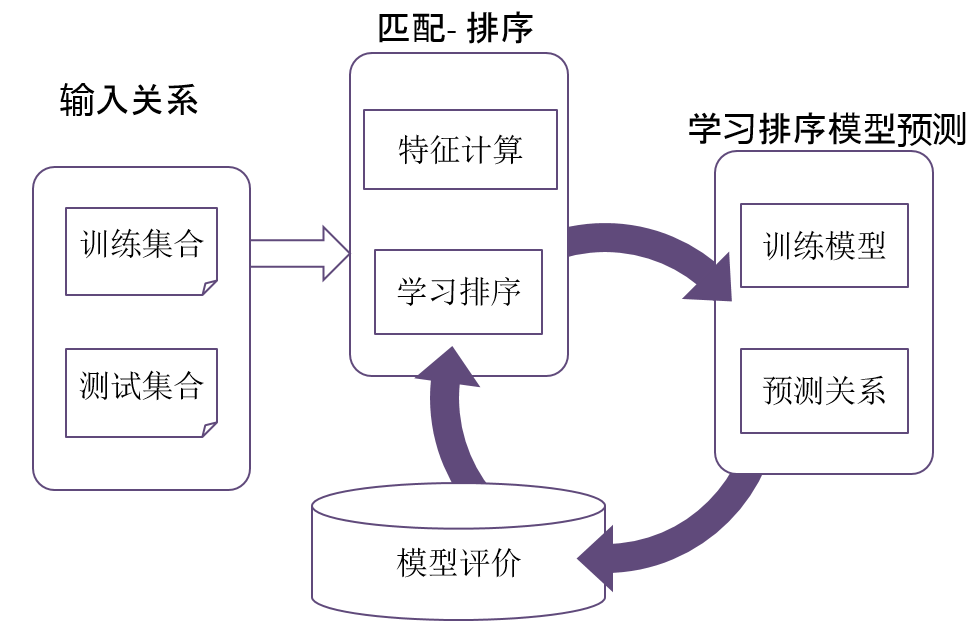
\includegraphics [width=0.5\textwidth]{frame.png}
\caption{一个知识库例子}
\label{frame}
\end{center}
\end{figure}
\section{特征计算}
特征计算是知识库补全的特征抽取阶段,特征的数量和特征有效性是决定知识库补全效果的关键点之一。
给定一个完整的知识库,我们将知识库中的实体和关系分别转化为图中的顶点和边,
这样就能构建一个基于图模型的知识库补全系统。对于知识库中每种待预测的关系,
我们抽取对应关系下的实体对,将实体对的头实体和尾实体在图中进行随机游走\cite{Lao2012},
获得连接头实体和尾实体的关系路径特征,从而获得了知识库补全的关系路径特征。
给定一个目标关系r和这个关系对应的实体对集合
$$I_s=\{(s_j,t_j)|<s_j,t_j> \in KB\}$$

我们期望找出连接头尾实体对的关系路径特征。
由于连接头尾实体对之间的路径数量很大,通常需要限定关系路径的长度,
并采用随机游走算法计算选择从头实体到尾实体的关系路径,将这些路径集合作为关系路径特征。
对于能连接从头实体到尾实体的关系路径,我们记录这个关系路径的类型,作为模型预测的特征。
我们计算0-1二值化后的的路径类型,作为关系路径特征的特征值。对于每个关系抽取的关系特征,我们最终记为$V_r$ $(h_i,t_i)$作为关系路径特征,表示从头实体到尾实体有哪些关系路径进行连接。
例如对于实体对“北京师范大学,位于,北京”三元组,我们可以基于上述的关系路径抽取算法获得
“北京师范大学,位于,北京市海淀区,位于,北京”、“北京师范大学,有校长,董奇,居住在,北京”等多条路径来
获得关系“位于”对应的关系路径类型特征。

本论文通过枚举不同维度的实体属性特征,计算这些实体对在这些实体属性特征下的特征值。
属性特征抽取过程较为复杂,不仅需要考虑不同维度的属性信息不一致问题,也要研究如何处理缺失值问题。
首先对于每个实体,有着不同类型的描述特征,如一个人的信息,不仅有出生年月这种时间类型的信息,
也有年龄、性别等不同种类的属性信息。我们采用了对实体信息进行标准化的方法,
将实体对的头实体和尾实体这些不同属性特征进行归一化处理范围限定在[0.1,1]之间。
进行标准化后计算获得新的属性特征记为$V_l(h_i)$和$V_l (t_i)$,分别表示头实体和尾实体在所有熟悉特征下的实体属性特征向量,其中$h_i$ 和$t_i$表示给定关系l的第i个头实体和尾实体,同时我们对于头实体和尾实体进行相减计算获得$V_l(h_i-t_i )$属性值。除此之外,对于很多实体在不同特征上的缺失值,我们将缺失值进行了补0处理,期望获得更优结果。
如对于“北京师范大学”这个实体,我们抽取了他的“建校时间”、“占地面积”等所有的实体属性特征,
并计算每个实体对在这些特征下标准化后的特征值,而且将缺失属性特征补0。

\section{模型预测}
对于上述\label{sec:literal}和\label{sec:relational}抽取到的关系路径特征和实体属性特征。
传统方法构建了一个分类器模型,学习每个关系和这个关系包含的实体对集合,将预测关系问题转化成一个分类预测问题。
$E_r=\{(h_i,t_j),y_i\}^N_{i=1} $表示关系r所有的实体对集合,其中$y_i\in \{0,1\}$,其中0表示负实体对,即知识库中并不是实际存在的三元组,
1表示正实体对,表示在知识库中实际存在的实体对,通过对知识库中的实体对进行分类器模型学习,
我们可以获得测试集合中实体对的打分情况。通常这个分类器采用逻辑回归算法进行模型的训练。
具体来说,对于每个关系的实体对,传统模型采用逻辑回归学习得到的关系路径特征向量$V_r$和实体属性特征向量$V_l$。
并定义了如下的逻辑回归函数,对每个关系下的实体对集合进行评价打分。
$$f(v,w)=\frac{1}{1+e^{w(V_r \oplus  V_l)}}$$
其中w表示关系路径特征和实体属性特征的学习权重参数。经典论文采用对数似然函数进行最大似然估计,
并通过随机梯度下降算法学习这些模型的参数,除此之外,还考虑到模型的过拟合和参数正则化表示,本论文定义了如下的
学习目标函数:
$$L_r=\frac{1}{N}\sum_{i=1}^N\{(y_ilog(f(v,w_r)) + (1-y_i)log(1-f(v,w_r))\}+\alpha ||w_r||+\beta||w_r^2||$$
其中,$L_r$表示给定关系r的目标函数,$\alpha$和$\beta$ 分别是$l_1$ 和$l_2$正则化惩罚项的权重,对于每个关系我们采用随机梯度下降算法使得整个训练集对数损失最小,同时结合$l_1$ 和$l_2$防止过拟合。最终我们可以学习得到每个关系下的关系路径特征和实体属性特征的权重。


\section{评价方式}
\label{sec:metrics}
知识库补全效果的评价方法和信息检索类似,主要采用MAP和MRR\cite{Gardner2014}指标进行模型评价。
在一个给定关系下,给定一个头实体和一系列的候选尾实体,我们希望排在前面的实体对是正确的实体对,
如果正例实体对排在负例实体对后面,则这个模型的预测效果有待改进。所有我们借鉴了信息检索领域相关的评价方法。

\subsection{平均准确率MAP}
平均准确率的英文全称是mean average precision。MAP的衡量标准比较单一,给定一个头实体和一系列候选尾实体,头尾实体对之间的关系非0即1,
我们采用局部封闭世界假设,在知识库中存在的实体对标记为1,即为正例,否则为负例。
MAP核心是利用头实体对应的相关的尾实体出现的位置来进行排序算法准确性的评估。
它反映系统在全部相关文档上性能的单值指标。系统模型计算出来的实体对越靠前(rank 越高),MAP就应该越高。否则准确率默认为0。MAP的计算公式如下:
$$MAP=\frac{\sum_{q=1}^nAP(q)}{n}$$
$$AP(q)=\frac{\sum_{i=1}^kP(i)\times rel(i)}{k}$$
其中MAP表示n个头实体和其候选尾实体的平均准确度的均值。AP(q)是一个头实体和其K个候选尾实体排序结果的评价,
如果正确的候选尾实体排在错误的候选尾实体之前,则AP值越高;
如果所有的头实体和其候选尾实体AP值越高,则模型的MAP值也就越高。
$rel(i)$在第i个实体对是预测结果时为1,否则为0。

\subsection{平均秩倒排序MRR}
MRR的全称是mean reciprocal rank。MRR通过定义第一个正确的候选尾实体来判断模型好坏,一个模型的MRR值越高,说明正确的候选尾实体在模型中排序越靠前。
MRR通常和MAP一起综合评价一个模型的好坏。
MRR的定义公式如下:
$$MRR=\frac{1}{n} \sum_{i=1}^n \frac{1}{r_i}$$

其中n表示一个关系下所有不同头实体的数目,$r_i$是每个头实体对应的正确尾实体的秩序。
MRR在很多基于问答系统的知识库补全系统\cite{West2014}中也是常见的评价方法之一。
通常情况下,基于符号逻辑的知识库补全系统中MRR值较高,多数实验结果都在0.9左右,大部分关系中的MRR实验结果差别不显著,
所以本研究的重点是关注如何显著提高知识库补全系统中关系补全的MAP指标。






% !Mode:: "TeX:UTF-8"
%%% Local Variables:
%%% mode: latex
%%% TeX-master: t
%%% End:

%实体属性和关系路径知识库补全

\chapter{关系和属性特征计算}
\label{cha:kbc-lit-relation}
本论文提供一种结合关系路径特征和实体属性特征的知识库补全方法。
通过提取知识库中实体的关系路径特征和实体属性特征,构建模型,进行知识库的实体关系预测。
除此之外,本论文研究了基于学习排序算法进行知识库补全的技术,在传统基于分类器模型的基础上,
提出了非线性的排序算法,对知识库候选实体对进行排序计算,获得更优的候选实体对排序集合。

\section{关系路径特征计算}
\label{sec:relational-compute}
特征计算是知识库补全的特征抽取阶段,特征的数量和特征有效性是决定知识库补全效果的关键点之一。
给定一个完整的知识库,我们将知识库中的实体和关系分别看做为图中的顶点和边,
这样就能构建一个基于图模型的知识库补全系统。对于知识库中每种特定待预测的关系,
我们抽取对应关系下的实体对,将实体对的头实体和尾实体在图中进行随机游走\cite{Lao2012},
获得连接头实体和尾实体的关系路径特征,从而获得了知识库补全的关系路径特征。
给定一个目标关系r和这个关系对应的实体对集合
$$I_s=\{(s_j,t_j)|<s_j,t_j> \in KB\}$$


\subsection{关系路径类型集合}
\label{sec:relational-set}
我们期望找出给定关系下,所有连接头尾实体对的关系路径特征,最终获得一个关系路径类型的集合。
在知识库中,由于连接头尾实体对之间的路径数量很大,通常需要限定关系路径的长度,一般限定图中的关系路径长度在2-6之间。

对于能连接从头实体到尾实体的关系路径,我们记录这个关系路径的类型,作为模型预测的特征。
我们采用随机游走算法\cite{Lovsz1993RandomWO}计算选择从头实体到尾实体的关系路径,将这些路径集合作为关系路径类型特征集合。
例如对于实体对“北京师范大学,位于(locatedIn),北京”三元组,我们可以基于上述的关系路径抽取算法获得
“北京师范大学,位于(locatedIn),海淀区,位于(locatedIn),北京”、“北京师范大学,有校长(hasPresident),董奇,居住在(livesIn),北京”等多条路径来
获得关系“位于”对应的关系路径特征,从而生成一个关系路径集合,包括两条不同的关系路径类型$\{locatedIn\to locatedIn, hasPresident \to livesIn\}$。对于反方向的关系路径我们采用${livesIn}^{-1}$表示。

\subsection{关系路径特征向量}
获取关系路径类型集合(记为S(r))后,我们将给定关系r下的实体对$(s_j,t_j)$计算所有关系路径类型集合下的特征值。
如果实体对$(s_j,t_j)$在集合S(r)中的某个关系路径$s_i$存在,则我们可以将该实体对的对应关系路径类型的特征值记为1,
否则该实体对在这个关系路径类型下的特征值记为0,这种算法简化了不同关系类型在知识库中的权重,但是一些实验表明\cite{Gardner2014}
进行0-1二值化可以简化关系路径类型特征和特征值计算过程,同时对于实验结果的影响并不显著。为了能在不影响模型效果的前提下,
加速我们的计算过程,我们对自己的关系路径类型特征值计算进行了0-1二值化。

\section{实体属性特征计算}
\label{sec:literal-compute}
除了\ref{sec:relational-compute}中计算得到的关系路径类型,考虑到在知识库中任然存在大量的实体属性特征并未被使用,
本研究也对每个关系下的实体属性特征进行计算,获得这些实体属性特征下的特征值。
实体属性特征获取较为简单,只需要枚举知识库中存在的不同实体属性类型,即可这些实体属性类型作为实体特征集合。
实体属性特征的处理和计算是获取更有效特征、提升知识库补全算法的关键。

属性特征抽取过程较为复杂,不仅需要考虑不同维度的属性信息不一致问题,也要研究如何处理缺失值问题。
本论文通过枚举不同维度的实体属性特征,计算这些实体对在这些实体属性特征下的特征值。
首先对于每个实体,有着不同类型的描述特征,如一个人的信息,不仅有出生年月这种时间类型的信息,
也有年龄、性别等不同种类的属性信息。我们采用了对实体信息进行标准化的方法,
将实体对的头实体和尾实体这些不同属性特征进行归一化处理范围限定在[0,1]之间。
进行标准化后计算获得新的属性特征记为$V_l(h_i)$和$V_l (t_i)$,分别表示头实体和尾实体在所有熟悉特征下的实体属性特征向量,其中$h_i$ 和$t_i$表示给定关系l的第i个头实体和尾实体,同时我们对于头实体和尾实体进行相减计算获得$V_l(h_i-t_i )$属性值。除此之外,对于很多实体在不同特征上的缺失值,我们将缺失值进行了补0处理,期望获得更优结果。
如对于“北京师范大学”这个实体,我们抽取了他的“建校时间”、“占地面积”等所有的实体属性特征,
并计算每个实体对在这些特征下标准化后的特征值,而且将缺失属性特征补0。

在对每个关系下的实体对集合进行实体属性特征抽取计算后,我们获得了这个关系下头实体的实体属性特征、尾实体的实体属性特征、
对头尾实体进行归一化后的归一化实体属性特征,以及头实体和尾实体差值计算得到的实体属性特征。

通过将\ref{sec:relational-compute}关系路径特征和\ref{sec:literal-compute}抽取的实体属性特征进行结合,我们获得了基于关系路径类型和实体属性类型的
特征矩阵,并构建机器学习模型对生成的特征矩阵进行学习预测,获得知识库补全中的实体对的关系。

\section{关系路径和实体属性特征实验}

\subsection{YAGO知识库实验}
\label{cha:exp-literal}
本部分的效果展示了在YAGO知识库下进行知识库补全算法的结果,我们的方法和对比方法被分为两组。
其中,SFE\_literal(图中简称SFE\_lit)和PRA\_literal(图中简称PRA\_lit)是结合关系路径特征和实体属性特征的方法,其MAP、MRR和AUC预测结果最好,
总体的预测结果最稳定,效果最好,而未加实体属性特征的PRA和SFE特征较好,
使用表示学习的TransE和TransR模型效果在MAP中预测较差,
但是通过AUC和hit@1进行模型的二分类效果结果和基于符号逻辑的效果相似。
结果显示,加入实体属性特征后,结合实体属性特征和关系路径特征的补全技术,相比只采用关系路径特征的补全技术有更高的准确性,在进行排序相关的预测效果评测时,有较好的效果。
在采用二分类模型进行评价时候,无论是符号逻辑的路径排序相关算法还是表示学习的低维嵌入算法,都能有效的进行模型预测。表\ref{tab:addlabel-kbcExp-data}中展示了YAGO和Freebase知识库的基本数据情况。

% Table generated by Excel2LaTeX from sheet 'Sheet2'
\begin{table}[htbp]
  \centering
  \caption{Add caption}
    \begin{tabular}{|l|r|r|}
    \hline
    \textcolor[rgb]{ .141,  .161,  .18}{} & \multicolumn{1}{l|}{FB15K} & \multicolumn{1}{l|}{YAGO} \\
    \hline
    实体    & 14951 & 58130 \\
    \hline
    关系类型  & 1345  & 32 \\
    \hline
    实体属性类型 & 336   & 25 \\
    \hline
    属性三元组 & 25776 & 141606 \\
    \hline
    关系三元组 & 592213 & 499350 \\
    \hline
    训练集   & 483142 & 399480 \\
    \hline
    测试集   & 59071 & 49132 \\
    \hline
    \end{tabular}%
  \label{tab:addlabel-kbcExp-data}%
\end{table}%

相比只采用关系路径的知识库补全算法,结合实体属性特征和关系路径特征的知识库补全算法,
在YAGO数据集合上,结果有较大的提升,相比原来的模型,SFE-literal和PRA-literal在计算MAP时,都获得了近1\%的效果提升,模型提升效果统计显著。
基于上述实验可以获得如下结论:(1)预测知识库中新三元组通过结合关系路径特征和实体属性特征能更加的精确有效,无论是以分类为优化目标的分类模型,还是以排序为优化目标的排序问题。
(2)由于在YAGO知识库集合中,有更多的属性事实进行关系预测,采用特征组合,能获得更多的不同类型组合特征,达到更好的优化结果,因此,结合属性事实和关系事实进行预测是非常重要的。
(3)对于某些特殊的关系,进行标准化处理是非常有效的,但是并非对于所有的属性事实进行标准化有效,选择合适的属性特征和实体关系特征进行组合是十分必要的。
(4)本研究的实验结果表明,对于多数YAGO2中的关系来说,我们的属性事实不仅可以用来预测关系事实,
而且还能调整原来的关系特征的路径权重,使得模型预测更加合理。
因此,结合属性事实和更丰富的关系特征能获得更好的知识库补全结果。
% Table generated by Excel2LaTeX from sheet 'yago'
% yago literal result
\begin{table}[htbp]
  \centering
  \caption{YAGO知识库实体属性和关系路径特征模型预测结果}
    \begin{tabular}{|l|r|r|r|r|}
    \hline
          & \multicolumn{1}{l|}{MAP} & \multicolumn{1}{l|}{MRR} & \multicolumn{1}{l|}{AUC} & \multicolumn{1}{l|}{hit@1} \\
    \hline
    SFE-lit & 78.610\% & 100.000\% & 92.994\% & 45.328\% \\
    \hline
    PRA-lit & 78.170\% & 97.830\% & 93.496\% & 45.104\% \\
    \hline
    PRA   & 77.610\% & 97.830\% & 93.258\% & 45.509\% \\
    \hline
    SFE   & 77.360\% & 97.830\% & 93.225\% & 45.502\% \\
    \hline
    transE & 56.400\% & 91.200\% & 92.740\% & 45.642\% \\
    \hline
    transR & 46.470\% & 65.410\% & 92.986\% & 46.128\% \\
    \hline
    \end{tabular}%
  \label{tab:addlabel}%
\end{table}%


我们进一步分析了每个关系下关系路径和实体属性特征的权重,表\ref{tab:lit-rel-kbc}显示了在YAGO知识库中的三种关系:Export、GraduateFrom、HasAcademicAdvisor,通过结合实体属性特征和关系路径特征,学习获得的重要权重。相比于路径排序算法这种只使用关系特征进行预测的方式,
结合属性事实特征不仅仅能增加模型预测的全面性,将模型预测结果精度提高,同时也能调整逻辑回归算法中不同关系路径特征和不同属性事实特征的权重。通过将关系路径特征和属性事实特征进行结合,使得模型的预测结果更加可靠。
如表所示,我们分析关系“graduateFrom”可以发现,除了常见的关系路径特征:
isCitizenOf $\to$ isCitizenOf$^{-1}$ $\to$ livesIn $\to$ isLocatedIn$^{-1}$、
isAffiliatedTo$^{-1}$ $\to$ isCitizenOf $\to$ livesIn $\to$ isLocatedIn$^{-1}$
等。
一些重要的实体属性特征如:wasCreatedOnDate、happenedOnDate等都在关系预测结果中有着重要的作用。通过分析这些关系路径的权重我们可以发现,实体属性特征不仅能提高关系预测中的精度,有较高的准确性,同时也能调整关系路径的权重,产生更多的有表达力的关系路径特征。

\begin{table}[htbp]
  \centering
  \caption{YAGO知识库关系路径和实体属性特征比较}
    \begin{tabular}{cp{12.3cm}|p{3.7cm}|}
    \hline
    \multicolumn{3}{c}{Export} \\
    \hline
    \multirow{5}[2]{*}{PRA} & imports$\to$ hasMusicalRole$^{-1}$$\to$ hasMusicalRole &  \\
          & livesIn$^{-1}$$\to$ diedIn$\to$ imports  &  \\
          & livesIn$^{-1}$$\to$ wasBornIn$\to$ dealsWith$^{-1}$ $\to$ imports &  \\
          & isCitizenOf$^{-1}$$\to$ influences$^{-1}$ $\to$ isCitizenOf$^{-1}$ $\to$ imports &  \\
          & isCitizenOf$^{-1}$$\to$ wasBornIn $\to$ dealsWith$^{-1}$ $\to$ imports &  \\
    \hline
    \multirow{5}[2]{*}{PRA-lit} & hasCapital $\to$ hasCapital$^{-1}$ $\to$ exports & hasGini \\
          & imports $\to$ hasMusicalRole$^{-1}$ $\to$ hasMusicalRole$^{-1}$ & hasInfaltion \\
          & isCitizenOf$^{-1}$ $\to$ wasBornIn $\to$ hasCapital$^{-1}$ $\to$ exports & hasEconomicGrowth \\
          & exports $\to$ hasMusicalRole$^{-1}$ $\to$ hasMusicalRole & hasPoverty \\
          & isInterestedIn$^{-1}$$\to$ wasBornIn $\to$ hasCapital$^{-1}$ $\to$ exports& wasDestroyedOnDate \\
    \hline
    \multicolumn{3}{c}{GraduateFrom} \\
    \hline
    \multirow{5}[2]{*}{PRA} & isCitizenOf $\to$ isCitizenOf$^{-1}$ $\to$ livesIn $\to$ isLocatedIn$^{-1}$&  \\
          & diedIn $\to$ happenedIn$^{-1}$ $\to$ participatedIn$^{-1}$ $\to$ isLocatedIn$^{-1}$ &  \\
          & hasWebsite $\to$ hasWebsite$^{-1}$ $\to$ livesIn $\to$ isLocatedin$^{-1}$ &  \\
          & isAffiliatedTo $\to$ isAffiliatedTo$^{-1}$ $\to$ isCitizenOf $\to$ isLocatedIn$^{-1}$ &  \\
          & isAffiliatedTo$^{-1}$ $\to$ isCitizenOf $\to$ livesIn $\to$ isLocatedIn$^{-1}$ &  \\
    \hline
    \multirow{5}[2]{*}{PRA-lit} & isAffiliatedTo $\to$ isAffiliatedTo$^{-1}$ $\to$ isCitizenOf $\to$ isLocatedIn$^{-1}$& happenedOnDate\\
          & hasAcademicAdvisor $\to$ hasAcademicAdvisor$^{-1}$ $\to$ graduatedFrom &wasDestroyedOnDate \\
          & hasWebsite $\to$ hasWebsite$^{-1}$ $\to$ livesIn $\to$ isLocatedin$^{-1}$ & wasDestroyedOnDate\\
          & isAffiliatedTo $\to$ isAffiliatedTo$^{-1}$ $\to$ isLeaderOf $\to$ isLocatedIn$^{-1}$ & wasCreatedOnDate \\
          & isCitizenOf $\to$ isCitizenOf$^{-1}$ $\to$ livesIn $\to$ isLocatedIn$^{-1}$ & wasBornOnDate \\
    \hline
    \multicolumn{3}{c}{HasAcademicAdvisor} \\
    \hline
    \multirow{5}[2]{*}{PRA} & wasBornIn $\to$ happenedIn$^{-1}$ $\to$ participatedIn$^{-1}$ $\to$ livesIn$^{-1}$ &  \\
          & diedIn $\to$ hasCapital$^{-1}$ $\to$ isLocatedIn$^{-1}$ $\to$ diedIn$^{-1}$ &  \\
          & worksAt $\to$ graduatedFrom$^{-1}$ $\to$ livesIn $\to$ wasBornIn$^{-1}$ &  \\
          & hasAcademicAdvisor $\to$ hasAcademicAdvisor$^{-1}$$\to$ influences$^{-1}$ $\to$ hasAcademicAdvisor &  \\
          & livesIn$\to$ diedIn $\to$ hasAcademicAdvisor &  \\
    \hline
    \multirow{5}[2]{*}{PRA-lit} & hasGender $\to$ hasGender$^{-1}$ & wasDestroyedOnDate \\
          & worksAt $\to$ graduatedFrom$^{-1}$ $\to$ livesIn $\to$ wasBornIn$^{-1}$ & hasHeight \\
          & hasAcademicAdvisor $\to$ hasAcademicAdvisor$^{-1}$ $\to$ diedIn $\to$ diedIn$^{-1}$ & hasHeight \\
          & diedIn $\to$ diedIn$^{-1}$ $\to$ livesIn $\to$ livesIn$^{-1}$ & wasBornOnDate \\
          & graduatedFrom $\to$ worksAt $\to$ worksAt$^{-1}$ $\to$ worksAt  & diedOnDate \\
    \hline
    \hline
    \end{tabular}%
  \label{tab:lit-rel-kbc}%
\end{table}%
% Table generated by Excel2LaTeX from sheet '工作表1'


\subsection{Freebase知识库实验}

本部分的效果展示了在Freebase知识库下进行知识库补全算法的结果,我们的方法和对比方法被分为两组,表\ref{tab:addlabel-fb}展示了在不同评价指标下Freebase知识库中部分关系的预测结果。
其中,SFE-literal和PRA-literal是结合关系路径特征和实体属性特征的方法,其MAP、MRR和AUC预测结果最好,
尤其在采用AUC进行模型评价时候,相比于表示学习方法,基于符号逻辑的知识库补全算法特征有非常高的提升。从基于MAP和MRR的评价指标来看,加入实体属性特征的总体预测结果最稳定,效果最好,而未加实体属性特征的PRA和SFE特征较好,
使用表示学习的TransE和TransR模型效果在MAP中预测较差,
结果显示,加入实体属性特征后,结合实体属性特征和关系路径特征的补全技术,相比只采用关系路径特征的补全技术有更高的准确性,在进行排序相关的预测效果评测时,有较好的效果。
在采用二分类模型进行评价时候,无论是符号逻辑的路径排序相关算法还是表示学习的低维嵌入算法,都能有效的进行模型预测。

% fb15k实验结果
\begin{table}[htbp]
  \centering
  \caption{Freebase知识库实体属性和关系路径特征模型预测结果}
    \begin{tabular}{|l|r|r|r|r|}
    \hline
          & \multicolumn{1}{l|}{MAP} & \multicolumn{1}{l|}{MRR} & \multicolumn{1}{l|}{AUC} & \multicolumn{1}{l|}{hit@1} \\
    \hline
    transR & 66.440\% & 95.500\% & 86.182\% & 44.145\% \\
    \hline
    transE & 72.910\% & 98.650\% & 89.118\% & 47.348\% \\
    \hline
    SFE   & 86.490\% & 98.650\% & 97.087\% & 55.559\% \\
    \hline
    SFE-lit & 86.560\% & 100.000\% & 97.140\% & 55.636\% \\
    \hline
    PRA   & 86.930\% & 98.200\% & 97.021\% & 55.527\% \\
    \hline
    PRA-lit & 87.140\% & 100.000\% & 97.108\% & 55.606\% \\
    \hline
    \end{tabular}%
  \label{tab:addlabel}%
\end{table}%

总体上看,使用MAP、MRR、AUC以及hit@1评价指标时,基于符号逻辑的知识库补全算法效果较基于表示学习的算法性能有较大的提升,而结合实体属性特征和结合关系路径特征的知识库补全算法相比仅仅使用关系路径特征的模型效果更好。这说明无论采用分类作为模型的优化方向,还是采用实体对排序的序列作为知识库补全优化目标,使用符号逻辑相比于近似的表示学习方法效果都有明显的提升。


分关系来看,从表\ref{tab:addlabel-fb-map}可以分析发现,在Freebase的15种关键关系中,
我们通过采用结合关系路径特征和实体属性特征的知识库补全算法,相比于只采用关系路径的知识库补全算法,我们的模型效果在MAP排序指标上有很大的提升。如/tv/tv/genreprograms、/filmactor/filmfilmperformancefilm 和 /film/director/film 、/media/commonnetflix/genretitles等关系使用MAP评测都有较大的模型效果提升。

% Table generated by Excel2LaTeX from sheet 'FB15K'
\begin{table}[htbp]
  \centering
  \caption{FB15K部分关系MAP得分}
    \begin{tabular}{|l|r|r|r|r|r|r|}
    \hline
    MAP-score & \multicolumn{1}{l|}{PRA-lit  } & \multicolumn{1}{l|}{PRA} & \multicolumn{1}{l|}{SFE-lit} & \multicolumn{1}{l|}{sfe} & \multicolumn{1}{l|}{transE} & \multicolumn{1}{l|}{transR} \\
    \hline
    /people/person/profession & 12.150\% & 11.902\% & 12.359\% & 12.096\% & 77.134\% & 71.784\% \\
    \hline
    /film/actor/film/film/performance/film & 28.309\% & 26.179\% & 22.121\% & 20.560\% & 87.007\% & 78.431\% \\
    \hline
    /media/common/netflix/genre/titles & 50.135\% & 48.281\% & 49.919\% & 49.546\% & 63.788\% & 65.603\% \\
    \hline
    /people/ethnicity/people & 57.143\% & 57.143\% & 57.143\% & 57.143\% & 60.402\% & 50.396\% \\
    \hline
    /film/film/genre/films/in/this/genre & 57.285\% & 55.650\% & 41.435\% & 41.828\% & 68.762\% & 64.254\% \\
    \hline
    /music/instrument/instrumentalists & 58.268\% & 58.268\% & 58.268\% & 58.268\% & 53.702\% & 52.452\% \\
    \hline
    /music/genre/artists & 69.514\% & 69.514\% & 69.514\% & 69.514\% & 77.745\% & 65.328\% \\
    \hline
    /location/location/time/zones & 77.479\% & 77.130\% & 77.479\% & 77.479\% & 82.790\% & 72.245\% \\
    \hline
    /tv/tv/genre/programs & 80.952\% & 80.952\% & 80.952\% & 80.952\% & 78.140\% & 60.484\% \\
    \hline
    /people/person/nationality & 81.119\% & 79.616\% & 81.774\% & 80.770\% & 75.448\% & 73.757\% \\
    \hline
    /people/cause/of/death/people & 82.653\% & 82.653\% & 82.653\% & 82.653\% & 52.979\% & 44.508\% \\
    \hline
    /music/record/label/artist & 83.704\% & 83.704\% & 83.704\% & 83.704\% & 55.037\% & 41.867\% \\
    \hline
    /film/production/company/films & 85.561\% & 85.561\% & 85.561\% & 85.561\% & 68.758\% & 59.189\% \\
    \hline
    /film/director/film & 100.000\% & 100.000\% & 100.000\% & 100.000\% & 94.077\% & 88.385\% \\
    \hline
    /film/film/directed/by & 100.000\% & 100.000\% & 100.000\% & 100.000\% & 95.254\% & 85.679\% \\
    \hline
    \end{tabular}%
  \label{tab:addlabel-fb-map}%
\end{table}%


我们以关系peoplepersonnationality和关系filmactorfilmfilmperformancefilm进行分析,研究关系路径特征和实体属性特征在路径排序算法中的特征表现。通过分析MAP指标来看,TransE和TransR这两个模型在各个关系上的效果较为稳定,符号逻辑相关算法在这些不同的关系上效果差别较大,通过分析相关的关系路径和实体属性权重,我们可以发现,这些关系路径特征相对于YAGO知识库来说,关系路径权重区别并不明显,甚至在结合实体属性特征后,对于filmactorfilmfilmperformancefilm这个关系来说,所有的关系路径和实体属性路径特征综合从44120减少到42787种特征。
说明基于随机游走抽取的关系路径特征并不能很好的区分Freebase中实体和实体之间的关系,
但是当加入关系路径特征后,能很好的惩罚这些加入区分度不好的关系路径特征。

其次尽管部分关系相对于表示学习来说,预测结果的效果较差,但是,基于图模型的知识库补全系统中,大部分关系的预测相对于基于表示学习效果提升很多。这一方面说明基于表示学习是一种近似的模型预测,而基于符号逻辑的关系路径学习排序则是一种精确而有效的学习方式。另一方面也说明,
在知识库构建的图模型中,部分关系较为稀疏的实体之间使用表示学习,预测结果较为理想,
而采用结合实体属性和关系路径的符号逻辑补全算法,则能基于有效的关系路径,获得十分有用的预测模型结果。

其次,由于Freebase知识库总共包含超过1345种不同类型的关系,这些关系覆盖了电影、人种、电视剧、音乐等不同类型的关系,这些不同的关系中部分关系具有对称性,一些关系和关系之间差别很大,
如何能将这些不同类型互不影响或者相互对称的关系区分出来,构建一个合理的图,基于这种合理的图模型进行关系路径的抽取和实体属性特征的计算,是未来研究的重要研究步骤。

\section{本章工作总结}
本部分通过抽取了实体属性类型、关系路径类型作为知识库补全的特征向量类型,并通过计算每个关系下实体对的实体属性特征值和关系路径特征值。将这些特征值进行组合,并构建了简单的逻辑回归算法模型,通过再不同知识库中的实验,评估了不同类型特征组合的情况下,我们结合关系路径特征和实体属性特征相比传统的关系路径特征计算问题,在分类预测、排序预测评估指标下的优势。

在接下来的章节中,本研究将通过构建不同的机器学习模型,通过比较逻辑回归分类算法、基于adaboost的树排序算法等来评估知识库补全算法应该如何选择预测模型。







% !Mode:: "TeX:UTF-8"

%%% Local Variables:
%%% mode: latex
%%% TeX-master: t
%%% End:

% 学习排序知识库补全
\chapter{知识库补全预测模型}

本部分基于抽取的实体属性特征和关系路径特征进行模型预测。模型预测主要分为两种方法:
分类模型和排序模型。传统的基于逻辑回归的分类算法对正负实体对进行分类模型学习,
利用二分类算法学习正负实体对的得分,依据得分大小将正负实体对进行划分,从而进行关系预测。
排序模型通过构建排序算法,对一组正负实体对进行学习排序,通过学习实体对的秩序排名,期望能将
正实体对排在负实体对之前,这样既可获得比传统分类回归算法更好的结果。本研究构建了基于树排序方法的
知识库补全算法和基于神经网络排序的知识库补全算法。
\label{sec:model}
\section{逻辑回归分类模型}
对于上述\label{sec:literal}和\label{sec:relational}抽取到的关系路径特征和实体属性特征。
传统方法构建了一个分类器模型,学习每个关系和这个关系包含的实体对集合,将预测关系问题转化成一个分类预测问题。
$E_r=\{(h_i,t_j),y_i\}^N_{i=1} $表示关系r所有的实体对集合,其中$y_i\in \{0,1\}$,其中0表示负实体对,即知识库中并不是实际存在的三元组,
1表示正实体对,表示在知识库中实际存在的实体对,通过对知识库中的实体对进行分类器模型学习,
我们可以获得测试集合中实体对的打分情况。通常这个分类器采用逻辑回归算法进行模型的训练。
具体来说,对于每个关系的实体对,传统模型采用逻辑回归学习得到的关系路径特征向量$V_r$和实体属性特征向量$V_l$。
并定义了如下的逻辑回归函数,对每个关系下的实体对集合进行评价打分。
$$f(v,w)=\frac{1}{1+e^{w(V_r \oplus V_l)}}$$
其中w表示关系路径特征和实体属性特征的学习权重参数。经典论文采用对数似然函数进行最大似然估计,
并通过随机梯度下降算法学习这些模型的参数,除此之外,还考虑到模型的过拟合和参数正则化表示,本论文定义了如下的
学习目标函数:
$$L_r=\frac{1}{N}\sum_{i=1}^N\{(y_ilog(f(v,w_r)) + (1-y_i)log(1-f(v,w_r))\}+\alpha ||w_r||+\beta||w_r^2||$$
其中,$L_r$表示给定关系r的目标函数,$\alpha$和$\beta$ 分别是$l_1$ 和$l_2$正则化惩罚项的权重,对于每个关系我们采用随机梯度下降算法使得整个训练集对数损失最小,同时结合$l_1$ 和$l_2$防止过拟合。最终我们可以学习得到每个关系下的关系路径特征和实体属性特征的权重。


\section{基于学习排序梯度下降树模型}
对于\label{sec:relational}中抽取的关系路径特征和\label{sec:literal}抽取的实体属性特征,我们需要构建基于学习排序算法的知识库补全模型进行关系训练和关系预测。
传统的路径排序算法中,当通过随机游走计算获得路径类型信息,并获得这些关系路径的值后,
再通过基于分类或者回归的算法,计算的到每个实体对的打分值,打分高的实体对排在打分低的实体对之前,
表示更可能是实际存在的实体对。而本技术不仅仅考虑实体对的打分高低,更关系实体对之间的排序关系,
正实体对总需要排序在负实体对前面,这样就能保证在预测的候选实体对中,总是排在前面的实体对是好的结果。
更具体的,我们采用一种学习排序的算法进行知识库补全。通过学习最小化实体对的pairwise损失函数,
直接优化MAP训练损失函数来进行模型参数更新,从而获得更好的模型预测结果。
我们使用基于LambdaMART的树的学习排序算法。对于一个给定的关系r,定义目标函数:
$$F(x_i|w,c)=\sum_{i=1}^K\alpha_i\pi(f_i)+\sum_{i=1}^Nl(f_i(x),f'_i(x))+\frac{C}{2}WW^T$$

其中第一项中的$\sum_{i=1}^K\alpha_i\pi(f_i)$是描述树复杂度的函数,总共有K个树进行模型训练。而第二项中$l(f_i(x),f'_i(x))$是模型的训练误差函数,
其中$f_i (x)$是每个实体对的实际分数,而$f'_i(x)$是通过模型学习得到的预测值,共训练了N轮,
训练误差函数可以根据实际需要改变,常见的训练误差函数可以选择MAP、AUC、NDCG等不同排序指标,
通常学习排序中MAP评价指标最为常见。考虑到我们目标函数是pairwise损失函数最小化,我们也选择MAP作为训练损失函数进行模型训练。
第三部分$\frac{C}{2}WW^T$是模型的惩罚项,是防止模型在训练数据中过拟合的L2惩罚函数。

\section{基于学习排序的知识库补全}
\label{cha:exp-relational}

展示了基于YAGO2的总体MAP和MRR进行模型评价的结果。我们可以看到基于学习排序的知识库补全技术相比传统的路径排序算法在MAP上有很大的提升,
基于学习排序的算法相比传统的算法在YAGO2数据集上有近50\%的效果提升;而四种方法在MRR指标上效果相当,
基于学习排序算法的MRR并未比传统路径排序算法有显著下降。

我们详细分析了37种YAGO2中关系的MAP指标,并在表 \ref{rank}展示了部分关系的MAP值。
分析可以发现,大部分关系采用学习排序算法后,预测结果有较大的提高,而在不同的关系类型预测中,
MAP差别较大,如:“playFor”和“isConnectedTo”等关系预测有较大的提高,而在“isInterestedIn”等关系中关系预测提升较差。
总体来说,有超过30种关系的MAP预测获得了显著的提升,只有不到5种关系MAP预测结果并未提升或略有下降,
这样的实验说明基于学习排序算法的知识库补全技术相比传统的分类回归打分模型有非常大的效果提升。

\begin{table}[htbp]
  \centering
  \caption{学习排序补全算法部分关系MAP值}
    \begin{tabular}{|l|r|r|r|r|}
    \hline
    relation & \multicolumn{1}{l|}{PRA} & \multicolumn{1}{l|}{SFE} & \multicolumn{1}{l|}{rankPRA} & \multicolumn{1}{l|}{rankSFE} \\
    \hline
    actedIn & 0.3379  & 0.3496  & 0.6222  & 0.6252  \\
    \hline
    created & 0.2523  & 0.2532  & 0.3089  & 0.3128  \\
    \hline
    dealsWith & 0.1729  & 0.1411  & 0.1265  & 0.1572  \\
    \hline
    graduatedFrom & 0.2646  & 0.2726  & 0.5607  & 0.5726  \\
    \hline
    hasCapital & 0.5637  & 0.6014  & 0.7275  & 0.7304  \\
    \hline
    hasChild & 0.5004  & 0.5078  & 0.6674  & 0.6757  \\
    \hline
    influences & 0.2946  & 0.2932  & 0.5771  & 0.5836  \\
    \hline
    isAffiliatedTo & 0.6364  & 0.6538  & 0.7816  & 0.7840  \\
    \hline
    playsFor & 0.6538  & 0.6606  & 0.8020  & 0.8036  \\
    \hline
    wasBornIn & 0.3661  & 0.3742  & 0.6053  & 0.6070  \\
    \hline
    worksAt & 0.2343  & 0.2281  & 0.5022  & 0.5014  \\
    \hline
    wroteMusicFor & 0.3488  & 0.3621  & 0.6144  & 0.6161  \\
    \hline
    \end{tabular}%
  \label{rank}%
\end{table}%

\section{本章工作总结}
本章中,我们主要比较了基于逻辑回归分类模型和基于adaboost的排序模型,
不同知识库补全模型中,我们可以发现基于排序的模型优化算法可以大幅提高正实体对
在所有实体对中的秩序,从而能改变原有的知识库补全优化中仅仅对实体对进行打分的模式,能够获得更好的预测效果。对于多数关系而言,进行逻辑回归的算法也较基于排序的算法效果差距明显。

%% !Mode:: "TeX:UTF-8"
%%% Local Variables:
%%% mode: latex
%%% TeX-master: t
%%% End:

\chapter{基于逻辑符号的知识库补全实验}
\label{cha:kbc-exp}
考虑到仅仅有部分的知识库系统同时拥有关系型三元组和属性型三元组,本文构建了一个基于YAGO的知识库补全实验。
\ref{cha:exp-literal}研究了如何在仅有关系路径特征的基础上,增加更多的实体属性特征,构建更好的知识库补全系统。
\ref{cha:exp-relational}研究了如何在传统的基于分类模型的基础上,采用基于学习排序的算法,构建实体对排序的秩序最优结果。


\section{YAGO知识库}
本研究构建了一个面向YAGO的知识库补全实例。YAGO是一个从维基百科上抽取的、包含地理名词、WordNet\cite{Kasneci2008TheYA}等数据的知识库。
YAGO将WordNet的词汇定义与维基百科的分类体系进行了融合集成\cite{Suchanek2008YAGOAL},使得YAGO具有更加丰富的实体分类体系。YAGO还考虑了时间和空间知识,为很多知识条目增加了时间和空间维度的属性描述。目前,YAGO包含1.2亿条三元组知识。YAGO是IBM Watson\cite{Ferrucci2010BuildingWA}的后端知识库之一。
而YAGO2是YAGO的一个实例,当前YAGO2包括超过千万的实体和超过1.2亿的实体知识,我们使用了其中实体的关系型三元组和属性型三元组共有4,484,914条、
37种关系型三元组的事实描述,同时有3,353,659条、35种属性性三元组的事实描述。

本研究中对于每种关系下的三元组,基于局部封闭世界假设,生成正负三元组。
对于每个正实体对,生成10个负实体对,其中5个随机替换头实体对,5个随机替换尾实体对。
在\ref{cha:exp-literal}中我们使用$YAGO_{all}$数据集。此外,我们还考虑到很多实体对缺少实体属性特征数据,在结合关系路径特征和实体属性特征中预测效果提升不明显,
因而采用算法过滤掉$YAGO_{all}$中缺失实体属性特征的实体对,构建了第二个知识图谱补全数据集合,称之为$YAGO_{lit}$。

\ref{cha:exp-relational}评测了路径排序算法(PRA)、子图特征抽取(SFE)两种常见的模型和基于学习排序的路径排序算法(rankPRA)、基于学习排序的子图特征抽取算法(rankSFE)在YAGO2的37种关系中的预测结果。
其中子图特征抽取是路径排序算法的一种拓展,相比传统路径排序算法,子图特征抽取算法能计算在特征计算上获得更多的路径特征。
基于学习排序算法的路径排序和子图特征抽取则在当前研究的基础上,改进模型的预测规则,将基于分类或回归的预测算法转化为基于排序的模型,
实验表明这样能更有效进行模型预测。模型评测的指标选取信息检索领域常见的指标MAP和MRR。

\section{关系路径特征和属性事实特征结合}
\label{cha:exp-literal}
本部分的效果展示了$YAGO_{all}$和$YAGO_{lit}$两种不同方法的结果,方法和对比方法被分为两组,PRA、$IRL_{pra}$ 、$IRL_{pra}^{nor}$和SFE、$IRL_{SFE}$ 、$IRL_{SFE}^{nor}$,在同一个组中使用相同的关系路径特征,我们在表格3中使用比较了不同的方法的平均精度即MAP在不同方法下的计算结果。
我们的结果显示,结合实体属性特征和关系路径特征的补全技术,相比只采用关系路径特征的补全技术有更高的准确性。


% Table generated by Excel2LaTeX from sheet 'Sheet1'
\begin{table}[htbp]
  \centering
  \caption{关系路径和实体属性特征的知识库补全的MAP结果}
    \begin{tabular}{|l|c|c|c|c|c|c|}
    \hline
    \multicolumn{1}{|c|}{} & \multicolumn{1}{l|}{PRA} & \multicolumn{1}{l|}{$IRL_{pra}$} & \multicolumn{1}{l|}{$IRL_{PRA}^{nor}$} & \multicolumn{1}{l|}{SFE} & \multicolumn{1}{l|}{$IRL_{sfe}$} & \multicolumn{1}{l|}{$IRL_{sfe}^{nor}$} \\
    \hline
    $YAGO_{all}$ & 0.4413 & 0.4635 & 0.4756 & 0.4643 & 0.4756 & 0.4729 \\
    \hline
    $YAGO_{lit}$ & 0.6128 & 0.6643 & 0.6632 & 0.6211 & 0.6823 & 0.669 \\
    \hline
    \end{tabular}%
  \label{tab:addlabel}%
\end{table}%


如表\ref{tab:addlabel}结果显示,结合实体属性特征的知识图谱补全方法相比于只基于路径特征的知识图谱补全方法,结果有较大的提升。在$YAGO_{all}$数据集合上,
$IRL_{pra}^{nor}$相比其他模型,有着较大的提升结果,在$YAGO_{lit}$数据集合上,结果显示$IRL_{SFE}$和$IRL_{SFE}^{nor}$ 都获得了非常显著的结果提升。同时$IRL_{pra}$获得了5\%的结果提升,而$IRL_SFE$ 获得了6\%的提升。
基于上述实验可以获得如下结论:预测知识库中新三元组通过结合关系路径特征和实体属性特征能更加的精确有效。
其次,由于$YAGO_{lit}$相比$YAGO_{all}$数据集合,有更加的多的属性事实进行关系预测,因此,结合属性事实和关系事实进行预测是非常重要的。
第三,对于某些特殊的关系,进行标准化处理是非常有效的,但是并非对于所有的属性事实进行标准化有效。
本发明的实验结果表明,对于多数YAGO2中的关系来说,我们的属性事实不仅可以用来预测关系事实,
而且还能调整原来的关系特征的路径权重,使得模型预测更加合理。
因此,结合属性事实和更丰富的关系特征能获得更好的知识库补全结果。

表\ref{tab:lit-rel-kbc}结果显示了三种关系的属性事实特征和关系路径特征。相比于路径排序算法这种只使用关系特征进行预测的方式,
结合属性事实特征不仅仅能增加模型预测的全面性,将模型预测结果精度提高,同时也能调整逻辑回归算法中不同关系路径特征和
不同属性事实特征的权重。通过将关系路径特征和属性事实特征进行结合,使得模型的预测结果更加可靠。
如表所示,我们分析关系“graduateFrom”可以发现,除了常见的关系路径特征:
isCitizenOf $\to$ isCitizenOf$^{-1}$ $\to$ livesIn $\to$ isLocatedIn$^{-1}$等。
一些重要的实体属性特征如:wasCreatedOnDate、happenedOnDate等都在关系预测结果中有着重要的作用。

\begin{table}[htbp]
  \centering
  \caption{属性特征和关系路径特征比较}
    \begin{tabular}{cp{12.6cm}|p{3.4cm}|}
    \toprule
    \multicolumn{3}{c}{Export} \\
    \midrule
    \multirow{5}[2]{*}{PRA} & imports$\to$ hasMusicalRole$^{-1}$$\to$ hasMusicalRole &  \\
          & livesIn$^{-1}$$\to$ diedIn$\to$ imports  &  \\
          & livesIn$^{-1}$$\to$ wasBornIn$\to$ dealsWith$^{-1}$ $\to$ imports &  \\
          & isCitizenOf$^{-1}$$\to$ influences$^{-1}$ $\to$ isCitizenOf$^{-1}$ $\to$ imports &  \\
          & isCitizenOf$^{-1}$$\to$ wasBornIn $\to$ dealsWith$^{-1}$ $\to$ imports &  \\
    \midrule
    \multirow{5}[2]{*}{IRL} & hasCapital $\to$ hasCapital$^{-1}$ $\to$ exports & hasGini \\
          & imports $\to$ hasMusicalRole$^{-1}$ $\to$ hasMusicalRole$^{-1}$ & hasInfaltion \\
          & isCitizenOf$^{-1}$ $\to$ wasBornIn $\to$ hasCapital$^{-1}$ $\to$ exports & hasEconomicGrowth \\
          & exports $\to$ hasMusicalRole$^{-1}$ $\to$ hasMusicalRole & hasPoverty \\
          & isInterestedIn$^{-1}$$\to$ wasBornIn $\to$ hasCapital$^{-1}$ $\to$ exports& wasDestroyedOnDate \\
    \midrule
    \multicolumn{3}{c}{GraduateFrom} \\
    \midrule
    \multirow{5}[2]{*}{PRA} & isCitizenOf $\to$ isCitizenOf$^{-1}$ $\to$ livesIn $\to$ isLocatedIn$^{-1}$&  \\
          & diedIn $\to$ happenedIn$^{-1}$ $\to$ participatedIn$^{-1}$ $\to$ isLocatedIn$^{-1}$ &  \\
          & hasWebsite $\to$ hasWebsite$^{-1}$ $\to$ livesIn $\to$ isLocatedin$^{-1}$ &  \\
          & isAffiliatedTo $\to$ isAffiliatedTo$^{-1}$ $\to$ isCitizenOf $\to$ isLocatedIn$^{-1}$ &  \\
          & isAffiliatedTo$^{-1}$ $\to$ isCitizenOf $\to$ livesIn $\to$ isLocatedIn$^{-1}$ &  \\
    \midrule
    \multirow{5}[2]{*}{IRL} & isAffiliatedTo $\to$ isAffiliatedTo$^{-1}$ $\to$ isCitizenOf $\to$ isLocatedIn$^{-1}$& happenedOnDate\\
          & hasAcademicAdvisor $\to$ hasAcademicAdvisor$^{-1}$ $\to$ graduatedFrom &wasDestroyedOnDate \\
          & hasWebsite $\to$ hasWebsite$^{-1}$ $\to$ livesIn $\to$ isLocatedin$^{-1}$ & wasDestroyedOnDate\\
          & isAffiliatedTo $\to$ isAffiliatedTo$^{-1}$ $\to$ isLeaderOf $\to$ isLocatedIn$^{-1}$ & wasCreatedOnDate \\
          & isCitizenOf $\to$ isCitizenOf$^{-1}$ $\to$ livesIn $\to$ isLocatedIn$^{-1}$ & wasBornOnDate \\
              \multicolumn{3}{c}{hasCurrency} \\
    \midrule
    \multicolumn{3}{c}{HasAcademicAdvisor} \\
    \midrule
    \multirow{5}[2]{*}{PRA} & wasBornIn $\to$ happenedIn$^{-1}$ $\to$ participatedIn$^{-1}$ $\to$ livesIn$^{-1}$ &  \\
          & diedIn $\to$ hasCapital$^{-1}$ $\to$ isLocatedIn$^{-1}$ $\to$ diedIn$^{-1}$ &  \\
          & worksAt $\to$ graduatedFrom$^{-1}$ $\to$ livesIn $\to$ wasBornIn$^{-1}$ &  \\
          & hasAcademicAdvisor $\to$ hasAcademicAdvisor$^{-1}$$\to$ influences$^{-1}$ $\to$ hasAcademicAdvisor &  \\
          & livesIn$\to$ diedIn $\to$ hasAcademicAdvisor &  \\
    \midrule
    \multirow{5}[2]{*}{IRL} & hasGender $\to$ hasGender$^{-1}$ & wasDestroyedOnDate \\
          & worksAt $\to$ graduatedFrom$^{-1}$ $\to$ livesIn $\to$ wasBornIn$^{-1}$ & hasHeight \\
          & hasAcademicAdvisor $\to$ hasAcademicAdvisor$^{-1}$ $\to$ diedIn $\to$ diedIn$^{-1}$ & hasHeight \\
          & diedIn $\to$ diedIn$^{-1}$ $\to$ livesIn $\to$ livesIn$^{-1}$ & wasBornOnDate \\
          & graduatedFrom $\to$ worksAt $\to$ worksAt$^{-1}$ $\to$ worksAt  & diedOnDate \\
    \midrule
    \bottomrule
    \end{tabular}%
  \label{tab:lit-rel-kbc}%
\end{table}%
% Table generated by Excel2LaTeX from sheet '工作表1'

\section{基于学习排序的知识库补全}
\label{cha:exp-relational}

展示了基于YAGO2的总体MAP和MRR进行模型评价的结果。我们可以看到基于学习排序的知识库补全技术相比传统的路径排序算法在MAP上有很大的提升,
基于学习排序的算法相比传统的算法在YAGO2数据集上有近50\%的效果提升;而四种方法在MRR指标上效果相当,
基于学习排序算法的MRR并未比传统路径排序算法有显著下降。

我们详细分析了37种YAGO2中关系的MAP指标,并在表 \ref{rank}展示了部分关系的MAP值。
分析可以发现,大部分关系采用学习排序算法后,预测结果有较大的提高,而在不同的关系类型预测中,
MAP差别较大,如:“playFor”和“isConnectedTo”等关系预测有较大的提高,而在“isInterestedIn”等关系中关系预测提升较差。
总体来说,有超过30种关系的MAP预测获得了显著的提升,只有不到5种关系MAP预测结果并未提升或略有下降,
这样的实验说明基于学习排序算法的知识库补全技术相比传统的分类回归打分模型有非常大的效果提升。


\begin{table}[htbp]
  \centering
  \caption{学习排序补全算法部分关系MAP值}
    \begin{tabular}{|l|r|r|r|r|}
    \hline
    relation & \multicolumn{1}{l|}{PRA} & \multicolumn{1}{l|}{SFE} & \multicolumn{1}{l|}{rankPRA} & \multicolumn{1}{l|}{rankSFE} \\
    \hline
    actedIn & 0.3379  & 0.3496  & 0.6222  & 0.6252  \\
    \hline
    created & 0.2523  & 0.2532  & 0.3089  & 0.3128  \\
    \hline
    dealsWith & 0.1729  & 0.1411  & 0.1265  & 0.1572  \\
    \hline
    graduatedFrom & 0.2646  & 0.2726  & 0.5607  & 0.5726  \\
    \hline
    hasCapital & 0.5637  & 0.6014  & 0.7275  & 0.7304  \\
    \hline
    hasChild & 0.5004  & 0.5078  & 0.6674  & 0.6757  \\
    \hline
    influences & 0.2946  & 0.2932  & 0.5771  & 0.5836  \\
    \hline
    isAffiliatedTo & 0.6364  & 0.6538  & 0.7816  & 0.7840  \\
    \hline
    playsFor & 0.6538  & 0.6606  & 0.8020  & 0.8036  \\
    \hline
    wasBornIn & 0.3661  & 0.3742  & 0.6053  & 0.6070  \\
    \hline
    worksAt & 0.2343  & 0.2281  & 0.5022  & 0.5014  \\
    \hline
    wroteMusicFor & 0.3488  & 0.3621  & 0.6144  & 0.6161  \\
    \hline
    \end{tabular}%
  \label{rank}%
\end{table}%








%%% 其它部分
%\backmatter

%
% % 参考文献
 \bibliographystyle{bnubib}
 \bibliography{ref/refs}

% 附录
%\begin{appendix}
%% !Mode:: "TeX:UTF-8"
%%% Local Variables:
%%% mode: latex
%%% TeX-master: "../main"
%%% End:

\chapter{其它附录}
前面两个附录主要是给本科生做例子。其它附录的内容可以放到这里,当然如果你愿意,可
以把这部分也放到独立的文件中,然后将其 \verb|\input| 到主文件中。 
%\end{appendix}
%
% % 学术成果
% % !Mode:: "TeX:UTF-8"
\begin{paper}
\begin{enumerate}
  \item Yong Huang, Zhichun Wang. Knowledge Base Completion by Learning to Rank Model. CCKS 2017:1-6
  \item Yong Huang, Zhichun Wang. Knowledge Base Completion using both Literal and Relational Facts. (EMNLP 在投)
  \item Zhichun Wang, Danlu Wen, Yong Huang, Chu Li.
Word, Mention and Entity Joint Embedding for Entity Linking. JIST (Workshops & Posters) 2016: 70-73
 \item Zhichun Wang, Rongyu Wang, Danlu Wen, Yong Huang, Chu Li.
Entity Linking in Queries Using Word, Mention and Entity Joint Embedding. JIST 2017: 138-150
  \item Jun Li, Jinxian Pan, Chen Ye, Yong Huang, Danlu Wen, Zhichun Wang. 
  Linking Entities in Chinese Queries to Knowledge Graph. NLPCC 2015: 590-597
  \item 黄勇,王志春。 基于学习排序算法的知识库补全方法及装置。(专利申请号:201810059641.2)
  \item 王志春,黄勇。 一种知识库的补全方法及装置。(专利申请号:201810085005.7)
  \end{enumerate}
\end{paper}


% 致谢
% !Mode:: "TeX:UTF-8"
%%% Local Variables:
%%% mode: latex
%%% TeX-master: "../main"
%%% End:

\begin{ack}
  衷心感谢导师王志春教授对本人的精心指导,他的言传身教将使我终生受益。

  在北京师范大学学习的三年中,承蒙王志春老师不辞劳苦的指导和帮助,让我从一个无知的年青人,
  慢慢学到很多做人做事做学问的道理,这些知识不仅仅帮助我在学术的道路上探索向前,也帮我
  成长,学会发现更大的世界。

  感谢我们实验室的所有师妹师弟们,感谢李楚同学不辞劳苦的帮助我解决Linux系统问题,感谢郑伟
  师妹帮我一起合作Java代码项目,感谢孙铭晨师妹经常为我们出谋划策,带给我们鲜美的水果零食,
  感谢吴妍蓉师妹帮我解决学术问题,带给我欢声笑语。最由衷的感谢我的父母,他们无私的为我付出,支持我在贫寒的
  学术道路上又坚持了三年,让我始终坚持自己的想法,做自己应该做的事情。

  感谢清华的薛瑞尼及相关同学,他们制作维护的清华学位论文模板极大的方便了\LaTeX{}用户的论文写作。

  最后附上苏轼的一首诗:{\kai 人生到处知何似,应似飞鸿踏雪泥。
  泥上偶然留指爪,鸿飞那复计东西。
  老僧已死成新塔,坏壁无由见旧题。
  往日崎岖还记否,路长人困蹇驴嘶。}
  人生匆匆,雪泥鸿爪。希望大家都能活的开心,做学问也开心。

\end{ack}


\end{document}
